\begin{frame}[fragile]
\frametitle{Automatic Dynamic Load Balancing}
\begin{itemize}
\item Measurement based load balancers
\begin{itemize}
\item Principle of persistence: In many CSE applications, computational loads and communication patterns tend to persist, even in dynamic computations
\item Therefore, recent past is a good predictor of near future
\item Charm++ provides a suite of load-balancers 
\item Periodic measurement and migration of objects
\end{itemize}
\item Seed balancers (for task-parallelism)
\begin{itemize}
\item Useful for divide-and-conquer and state-space-search applications
\item Seeds for charm++ objects moved around until they take root
\end{itemize}
\end{itemize}
\end{frame}

\begin{frame}[fragile]
\frametitle{Using the Load Balancer}
\begin{itemize}
\item link a LB module 
\begin{itemize}
\item \code{-module <strategy>}
\item RefineLB, NeighborLB, GreedyCommLB, others…
\item EveryLB will include all load balancing strategies
\end{itemize}
\item compile time option (specify default balancer)
\begin{itemize}
\item \code{-balancer RefineLB}
\item runtime option
\item \code {+balancer RefineLB}
\end{itemize}
\end{itemize}
\end{frame}

\begin{frame}
\frametitle{Code to Use Load Balancing}
\begin{itemize}
\item Insert \code{if (myLBStep) AtSync() else ResumeFromSync();} call at natural barrier
\item Implement \code{ResumeFromSync()} to resume execution
\begin{itemize}
\item Typical ResumeFromSync contribute to a reduction
\end{itemize}
\end{itemize}
\end{frame}

\begin{frame}
\frametitle{Performance}
\begin{centering}
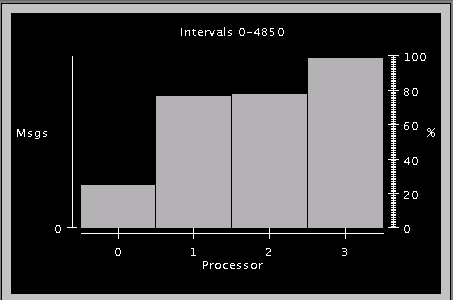
\includegraphics[width=0.5\textwidth]{figures/beforeLB}
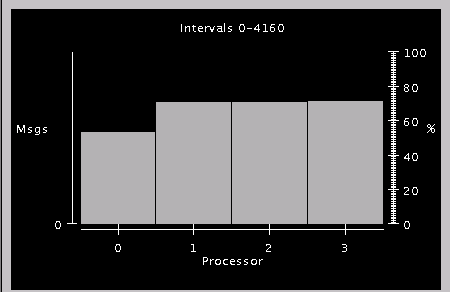
\includegraphics[width=0.5\textwidth]{figures/afterLB}
\end{centering}
\end{frame}
